%------------------------------------------------------------------------------
% Template file for the submission of papers to IUCr journals in LaTeX2e
% using the iucr document class
% Copyright 1999-2013 International Union of Crystallography
% Version 1.6 (28 March 2013)
%------------------------------------------------------------------------------

\documentclass[preprint]{iucr}              % DO NOT DELETE THIS LINE

     %-------------------------------------------------------------------------
     % Information about journal to which submitted
     %-------------------------------------------------------------------------
     \journalcode{J}              % Indicate the journal to which submitted
                                  %   A - Acta Crystallographica Section A
                                  %   B - Acta Crystallographica Section B
                                  %   C - Acta Crystallographica Section C
                                  %   D - Acta Crystallographica Section D
                                  %   E - Acta Crystallographica Section E
                                  %   F - Acta Crystallographica Section F
                                  %   J - Journal of Applied Crystallography
                                  %   M - IUCrJ
                                  %   S - Journal of Synchrotron Radiation
\usepackage{graphicx}
\usepackage[T1]{fontenc}
\usepackage[utf8]{inputenc}
\usepackage{amsmath}

\begin{document}                  % DO NOT DELETE THIS LINE

     %-------------------------------------------------------------------------
     % The introductory (header) part of the paper
     %-------------------------------------------------------------------------

     % The title of the paper. Use \shorttitle to indicate an abbreviated title
     % for use in running heads (you will need to uncomment it).

\title{Application of signal separation to diffraction image compression and serial crystallography}
%\shorttitle{Short Title}

     % Authors' names and addresses. Use \cauthor for the main (contact) author.
     % Use \author for all other authors. Use \aff for authors' affiliations.
     % Use lower-case letters in square brackets to link authors to their
     % affiliations; if there is only one affiliation address, remove the [a].

\cauthor[a]{Jérôme}{Kieffer}{jerome.kieffer@esrf.fr}{}
\author[a]{Nicolas}{Coquelle}
Samuel
Alejandro
\author[a]{Gianluca}{Santoni}
shibom
\author[a]{Jonathan P.}{Wright}
\author[a]{Gavin}{Vaughan}
\author[a]{Daniele}{De Sanctis}
\aff[a]{European Synchrotron Radiation Facility;71, avenue des Martyrs;CS 40220;38043 Grenoble Cedex 9 \country{France}}

     % Use \shortauthor to indicate an abbreviated author list for use in
     % running heads (you will need to uncomment it).

%\shortauthor{Soape, Author and Doe}

     % Use \vita if required to give biographical details (for authors of
     % invited review papers only). Uncomment it.

%\vita{Author's biography}

     % Keywords (required for Journal of Synchrotron Radiation only)
     % Use the \keyword macro for each word or phrase, e.g. 
     % \keyword{X-ray diffraction}\keyword{muscle}

%\keyword{keyword}

     % PDB and NDB reference codes for structures referenced in the article and
     % deposited with the Protein Data Bank and Nucleic Acids Database (Acta
     % Crystallographica Section D). Repeat for each separate structure e.g
     % \PDBref[dethiobiotin synthetase]{1byi} \NDBref[d(G$_4$CGC$_4$)]{ad0002}

%\PDBref[optional name]{refcode}
%\NDBref[optional name]{refcode}

\maketitle                        % DO NOT DELETE THIS LINE

\begin{synopsis}
Precise background assessment and application to single crystal image compression and serial crystallography data reprocessing. 
\end{synopsis}

\begin{abstract}
Abstract goes here.
\end{abstract}


     %-------------------------------------------------------------------------
     % The main body of the paper
     %-------------------------------------------------------------------------
     % Now enter the text of the document in multiple \section's, \subsection's
     % and \subsubsection's as required.

\section{Introduction}

%\cite{Cheetah2014}
The Synchrotron serial crystallography beamline (ID29 at ESRF) has been built to \ldots
In this setup samples will be carried in front of the beam and a Jungfrau 4M detector records 


\section{Algorithm for the separation of amorphous background from Bragg peaks}
\subsection{Background scattering}
The core idea of the separation of Bragg peaks from background is to consider that the background scattering 
is originating from unordered matter which gives some isotropic signal, preferably with smooth variations.
For this the raw signal has to be corrected from dark noise and any systematic anisotropic effects like polarization corrections.

The initial implementation in pyFAI \cite{pdj2013} relied on a 2D radial transform followed by a median filter in the azimuthal dimension 
to separate amorphous scattering from crystalline scattering.
Despite this method has been successfully used for large dataset analysis \cite{brocades}, it has several major drawbacks:
* The 2D averaging mixes the signal of several pixels and blurs the signal. 
* Pixel-splitting is needed to leverage the moiré effect in the 2D averaging, but this increases further the blurring. 
* The filtered 1D curve obtained after the median shows sharp jumps from one azimuthal bin to its neighbor.
* Median filter is complicated and requires a lot of memory.
    
The coming sections present an efficient way to perform the azimuthal averaging and the associated variance propagation, 
and how it can be used to perform the statistical analysis to extract the background from a diffraction image. 

\subsection{Efficient azimuthal averaging and uncertainties evaluation}

\subsubsection{Preprocessing} is a pixel-wise correction for dark current and several normalization corrections\cite{pyfai_2020} which is described in Equation\ref{norm}:
\begin{equation}
\label{norm}
I_{cor} = \frac{signal}{norm}  = \frac{I_{raw} - I_{dark}}{F \cdot
\Omega \cdot P \cdot A \cdot I_0} 
\end{equation}
where the numerator ($signal$ hereafter) is the subtraction of the $I_{dark}$ is the dark current from the the detector's raw signal $I_{raw}$.
The denominator (hereafter $norm$) is a normalization factor composed of the product of  $F$:  a factor accounting for the flat-field correction, $\Omega$: the solid
angle subtended by a given pixel, $P$: the polarisation correction term and
$A$: the detector's apparent efficiency due to the incidence angle of the
photon on the detector (for integrating detectors, high energy photons with
larger incidence angle see larger sensor thickness, and thus have higher
detection probability).
Intensity can also be normalized by the incoming flux $I_0$, which is independent of the pixel position.

\subsubsection{Azimuthal averaging} was initially implemented using histograms and since the the geometry of the experimental setup was fixed during the acquisition, a look-up table listing all pixels contributing to each  azimuthal bin could be built and used to speed-up calculations \cite{pyFAI_gpu}.
The azimuthal transformation being a linear transformation, it can be implemented as a  matrix multiplication with a sparse-matrix representing the transformation and the a dense vector which is simply the flattened view of the diffraction image. 
The CSR sparse matrix representation is preferred since it is very efficient to perform dot products with dense vectors.
The coefficients $c_{i,r}$ of the matrix are the fraction of area of a pixel $i$ falling into the bin $r$.
In the case where pixel splitting is deactivated those coefficients  ($c_{i,r}$) are always one (and zero elsewhere) since each pixel contribute to a single bin.
The sparse matrix multiplication can be used to sum efficiently values for all pixels belonging to the same bin.
The summed signal divided by the summed normalization provides the intensity averaged over all pixels falling in the bin at the distance $r$ from the center, Eq\ref{avg}: 
\begin{equation}
\label{avg}
<I>_{r} = \frac{\sum\limits_{i \in bin_r} c_{i,r} \cdot signal_i}
                        {\sum\limits_{i \in bin_r} c_{i,r} \cdot norm_i} 
\end{equation}  

\subsubsection{Uncertainty evaluation from Poisson law.}
Photon counting suffered from several uncertainties, among which the most important one is usually the counting statistics (often referred as Poisson law)
stating that the variance for a pixel is at least the number of events counted.
Other sources of noise superimposes quadratically to the Poisson noise, like the dark-current noise as preented in Eq\ref{poisson}:     
\begin{equation}
\label{poisson}
var(I) = (\sigma(I))^{2} = I_{raw} + (\sigma_{dark})^{2}  
\end{equation}
During the regrouping part, the coefficients of the sparse matrix needs to be squared for the numerator to have uncertainties $\sigma$ proportional to the raw signal, Eq\ref{varianceP}.
\begin{equation}
\label{varianceP}
(\sigma_{r}(I))^2 = \frac{\sum\limits_{i \in bin_r} c_{i,r}^2 \cdot var_i}
                  {\sum\limits_{i \in bin_r} c_{i,r} \cdot norm_i} 
\end{equation}
One should distinguish the \textit{uncertainty of the mean} (sometimes referred are standard error of the mean or $sem$) 
which describes the precision with which the mean is known (and described in \cite{pyfai_2020}),
from the \textit{uncertainty of the pixel value} (often referred are standard deviation, $std$). 
Those two value differ only by square root of the number of measurements: $sem = std/\sqrt{norm}$.
Thus, the more data point, the more precisely is known the mean value.
Since this document focuses on the uncertainties of pixel values, the \textit{standard deviation} will systematically be used in this document.  

\subsubsection{Uncertainty evaluation from variance in a bin.}
When considering the diffraction of an isotropic compound (liquid, amorphous or perfect powder), all pixels falling into the same radial bin should see the same flux of photons and the deviation to their intensities could be used to estimate the uncertainty.
Variance (and standard deviation) are usually obtained in a two steps procedure: one pass to calculate the average value (Eq\ref{avg})and a second to calculate the deviation to the average (Eq\ref{varA}. 
This double pass approach can be implemented using sparse matrix multiplication but requires the access of each pixel twice and extra storage space, but it is very stable numerically.
\begin{equation}
\label{varA}
(\sigma_{r}(I))^2 = \frac{\sum\limits_{i \in bin_r} c_{i,r} \cdot norm_i \cdot (\frac{signal_i}{norm_i}-<I>_r)^2}
                         {\sum\limits_{i \in bin_r} c_{i,r} \cdot norm_i}  ?=  \sum\limits_{i \in bin_r} c_{i,r} \cdot  (\frac{signal_i}{norm_i}-<I>_r)^2
\end{equation}


 
Single pass implementation of variance are faster since they access pixels only once and offer the ability to perform parallel reductions, i.e. work with blocks of pixels.
\citeasnoun{variance2018} presents a complete review, with some key equations reported and adapted to the formalism of crystallography hereafter.
For example the weight for a pixel is $\omega_i = c_i \cdot normalization_i$
If $P$ is a partition of the ensemble of pixels falling into a given azimuthal bin, let $\Omega_{P}$, $V_{P}$ and $VV_{P}$  
be the weight sum, the weighted sum of $V$ and the weighted sum of deviation squared over the partition $P$: 
\begin{equation}
\Omega_{P} = \sum\limits_{i \in P} \omega_i = \sum\limits_{i \in P} c_i \cdot norm_i 
\end{equation}
\begin{equation}
V_{P} = \sum\limits_{i \in P} \omega_i \cdot v_i =  \sum\limits_{i \in P} c_i \cdot signal_i
\end{equation}
\begin{equation}
VV_{p} = \sum\limits_{i \in P} \omega_i \cdot (v_i - V_{P}/\Omega_{P})^2 
\end{equation}

The average and the variance are then expressed as:
\begin{equation}
<I>_P = V_{P}/\Omega_{P} =  \frac{\sum\limits_{i \in P} c_i \cdot signal_i}
                        {\sum\limits_{i \in P} c_i \cdot norm_i} 
\end{equation}

\begin{equation}
(\sigma_P(I))^2 = VV_{P}/\Omega_{P} 
\end{equation}

Performing the union of two partition $A$ and $B$ allows the parallel reduction, which is especially efficient on GPU:
\begin{equation}
\Omega_{A \cup B} =  \Omega_{A} + \Omega_{B} 
\end{equation}

\begin{equation}
V_{A \cup B} =  V_{A} + V_{B} 
\end{equation}
  
\begin{equation}
VV_{A \cup B} =  VV_{A} + VV_{B} +  \frac{(\Omega_{A} \cdot V_{B} - \Omega_{B}\cdot V_{A})^2}{V_{A \cup B} \cdot  V_{A} \cdot V_{B}}
\end{equation}
  
The numerical stability issue is addressed by using double-precision arithmetic when implemented on CPU and double-word arithmetic when running on GPU \cite{double_word}.

\subsection{Histogram intensity }

The figure \ref{fig1}a presents the diffraction from a single crystal of insulin and several curves obtained from azimuthal integration: 
\ref{fig1}b is the azimuthally integrated signal (blue curve). Bragg peaks are seen as spikes on top of the background.
The plot \ref{fig1}c presents the uncertainties measured according to the Poisson law (orange curve, valid since the Pilatus is a photon counting detector) 
or the deviation in the ring (blue curve), much larger value since Bragg peaks contribute a lot to the deviation despite they represent few pixels.         
In the plot \ref{fig1}d are presented histogram of pixel intensity for  pixel laying at 80mm and 160mm from the beam center. 
Each of those histograms is composed of a bell-shaped distribution, centered on the average value with negative outliers tagged with the pixel value -1
(this is specific to the Pilatus detector), and few positive outliers which are usually Bragg peaks.   
Those histograms in figure \ref{fig1}d have been fitted with a Gaussian curve and both the center ($\mu$) and the width ($\sigma$) of the curve match 
roughly with the average (in \ref{fig1}b) and uncertainties (in \ref{fig1}c).  
\begin{figure}
\label{fig1}
\begin{center}
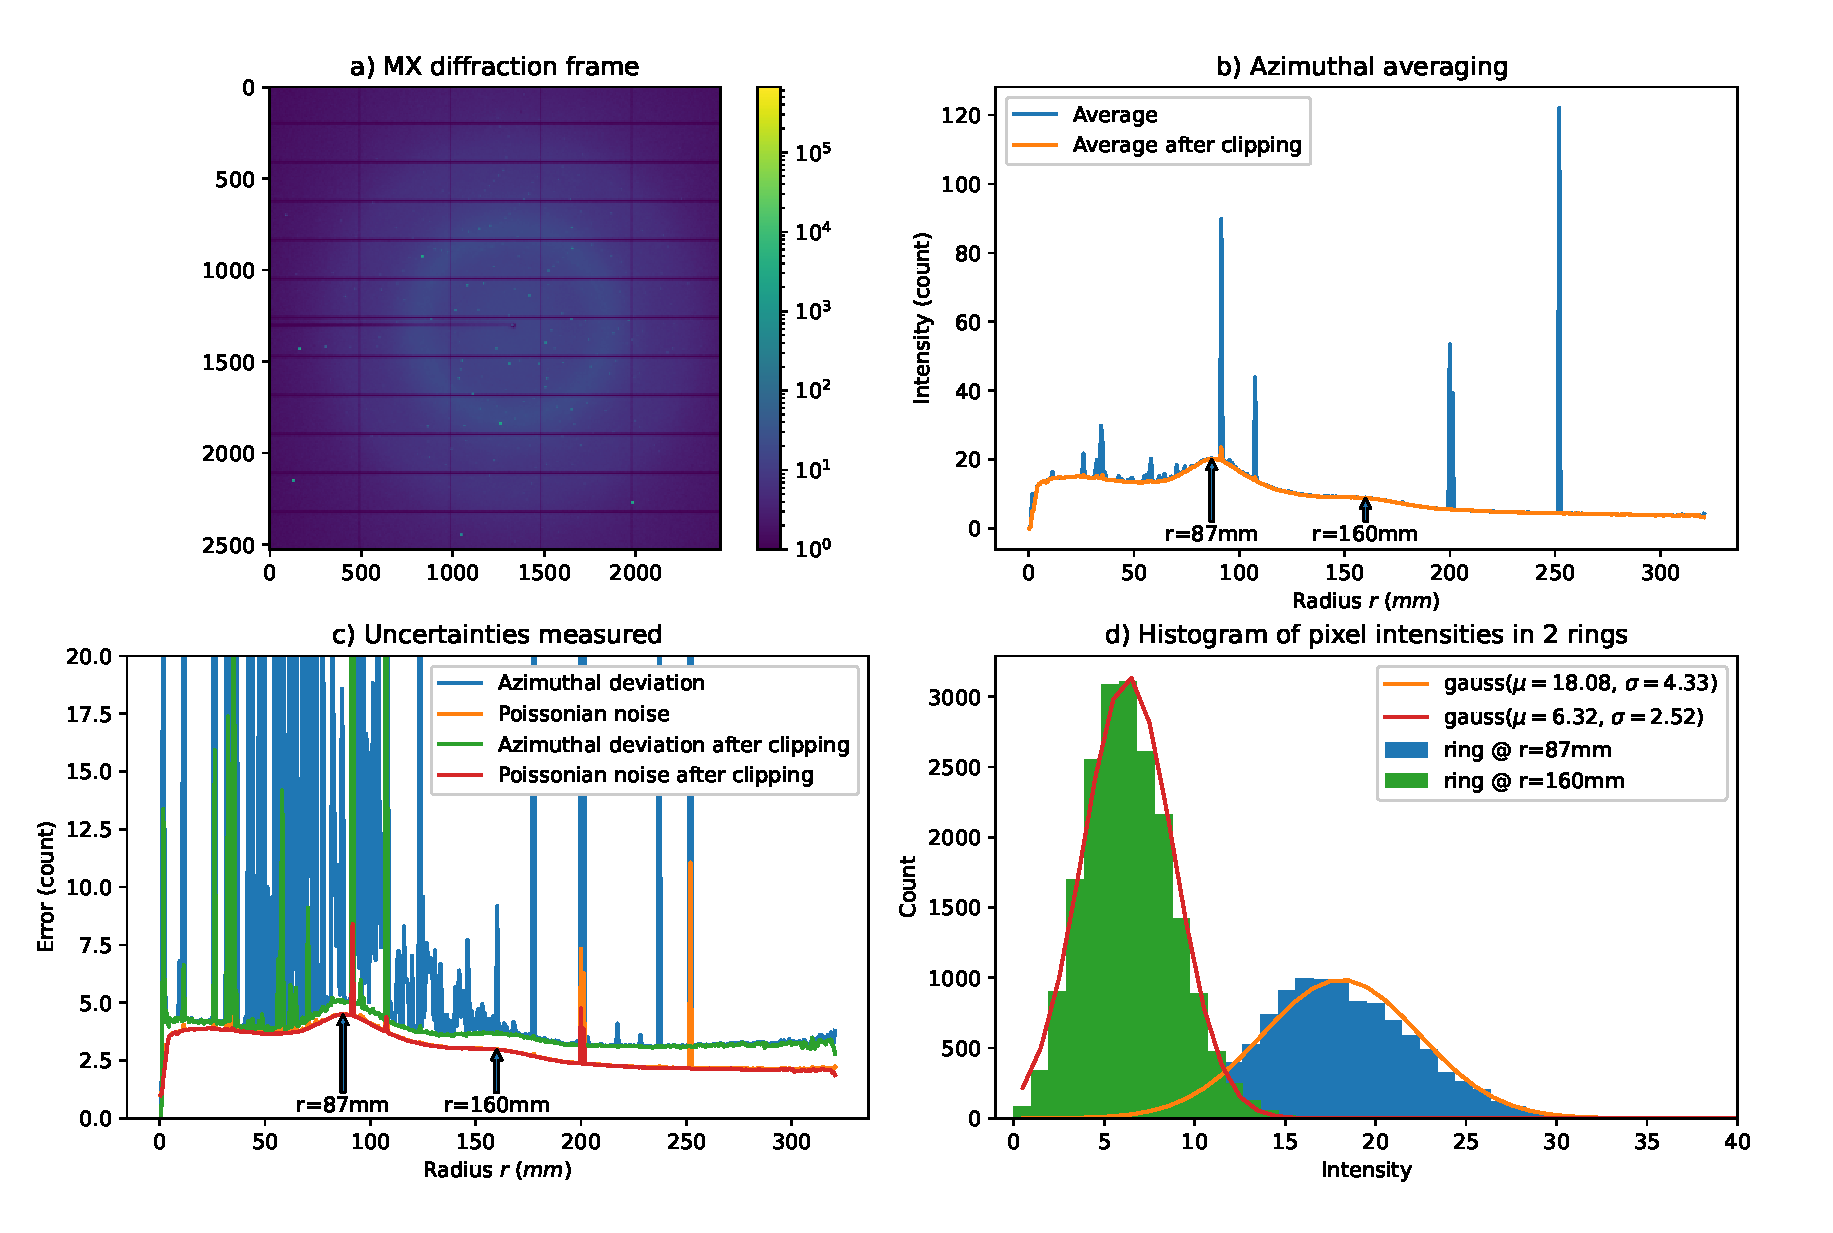
\includegraphics[width=14cm]{fig1}
\caption{Single crystal diffraction frame obtained from insulin with a Pilatus6M (a) (part of Dectris's reference dataset) with the azimuthally averaged signal (b), 
before and after clipping data. Uncertainties are presented in (c) when calculated assuming a Poissonian error model or when measuring the deviation within all pixels in a ring.
Subplot (d) presents the histogram of intensities for two rings at r=80mm and r=160mm from beam center with the distribution fitted as Gaussians.}
\end{center}
\end{figure}

The core idea of the algorithm for background extraction is to model the distribution of background pixels. Unlike Bayesian statistics \cite{Sivia2006} where the cost function is usually tuned to weight less outlier, here, those outliers are simply flagged and discarded.
Positive outliers can reasonably be assigned to Bragg peaks and negative outliers to shadows or defective pixels. 
The distribution is recalculated  after discarding pixels which intensity differ from the average value by more than $n$ times the standard deviation (Eq\ref{clip}) which has the effect of re-centering the distribution and enforcing a normal distribution of the remaining values:
\begin{equation}
\label{clip}
|I - <I>| > n \cdot \sigma(I)
\end{equation}
The orange plot in figure \ref{fig1}b presents the average after having discarded those outliers, and the orange and green curve of figure \ref{fig1}c are the uncertainties calculated after this clipping. 
 After clipping the average and uncertainties curves have lost most of their spikes, which means that Bragg peaks and shadowed pixel were discarded.
 
\subsection{Sigma-clipping}
The \textit{sigma-clipping} algorithm consists in iteratively applying the outlier rejection previously described and thus enforces the background distribution to follow a normal law.
There are two parameters to this algorithm: the number of iterations of clipping and the rejection cut-off.

\subsubsection{Number of iterations:}
Despite the execution time is proportional to the number of iteration of sigma-clipping, iterations should continue until no more outliers are found and the 
background distribution actually matches a Gaussian distribution. 
Since the loop exits as soon as no more outliers were discarded at the clipping step, having an arbitrary large number of iteration is not an issue for the execution time and the number of actual iteration is usually few (3 is commonly observed).       

\subsubsection{Clipping threshold:}
This threshold can be automatically calculated based on a variation on Chauvenet's criterion \cite{chauvenet} where one would accept to discard only a single pixel in a ring with a signal already following a normal law. 
Thus, the threshold value is adapted to the $size$ of the distribution, i.e. the number of pixels in each ring (Eq\ref{chauvenet}), which can reach several thousands and shrinks with iterations.
Typically the numerical value for this cut-off varies from 2 to 4.   
\begin{equation}
\label{chauvenet}
SNR_{chauvenet} =  \sqrt{2 log(\frac{size}{\sqrt{2 \pi}})}
\end{equation}

\section{Application to single crystal diffraction image compression}
Single crystal diffraction images exhibit usually an isotropic background on top of which are Bragg peaks.
The sigma-clipping algorithm can be used to select the background level and more importantly the associated uncertainty.

This lossy compression algorithm consists in picking (and storing) pixels which intensity is above the background value plus $p$ standard deviation. This value $p$ controls the amount of data to store and provides also an upper level for the compression ratio obtained since with $p=1$, 16\% of the pixel are stored but only 2.4\% for $p=2$ and 0.15\% for $p=3$. 
Stored pixels need to record not only the intensity but also the position. 
Moreover, to be able to regenerate the background, the averaged and uncertainties curves needs to be stored. 
\subsection{Sparsification}

\subsection{Densification}

\subsection{Quality}

\subsection{Performances}

\section{Application to serial crystallography}

\subsection{Performance}
     % comparison with cheetah
\section{Conclusion}
drawback: textured background

     %-------------------------------------------------------------------------
     % The back matter of the paper - acknowledgements and references
     %-------------------------------------------------------------------------

     % Acknowledgements come after the appendices

\ack{Acknowledgements}



\bibliographystyle{iucr}
\bibliography{biblio}

\end{document}                    % DO NOT DELETE THIS LINE
%%%%%%%%%%%%%%%%%%%%%%%%%%%%%%%%%%%%%%%%%%%%%%%%%%%%%%%%%%%%%%%%%%%%%%%%%%%%%%
